\documentclass[a4paper, 12pt]{article}
\usepackage{titling}
\usepackage{amsmath, amssymb, physics}
\usepackage{chngpage}
\usepackage{multirow}
\usepackage{graphicx}
\usepackage{titlesec}
\usepackage{fancyhdr}
\usepackage{chngcntr}
\graphicspath{ {figs/} }
\usepackage{indentfirst}
\usepackage{relsize}
\usepackage[margin=3cm]{geometry}
\usepackage{multirow}
\usepackage[table,xcdraw]{xcolor}
\usepackage{hhline}
\usepackage{titletoc}
\usepackage{afterpage}
\usepackage{caption} 
\usepackage{float}
\usepackage{listings}
\captionsetup[table]{skip=10pt}

\lstset{
    language=Python,
    literate={á}{{\'a}}1
        {ã}{{\~a}}1
        {é}{{\'e}}1
        {ó}{{\'o}}1
        {í}{{\'i}}1
        {ñ}{{\~n}}1
        {¡}{{!`}}1
        {¿}{{?`}}1
        {ú}{{\'u}}1
        {Í}{{\'I}}1
        {Ó}{{\'O}}1
}

\setlength{\droptitle}{-15em}


\pagestyle{fancy}
\fancyhf{}
\fancyhead[L]{Control de un motor de C.C.}
\fancyhead[R]{M. de Miguel}
\fancyfoot[c]{\thepage}

\newcommand\blankpage{%
	\null
	\thispagestyle{empty}%
	\addtocounter{page}{-1}%
	\newpage}

\renewcommand{\figurename}{Figura}
\renewcommand{\contentsname}{Índice}

\begin{document}
	\begin{titlepage}
		\centering
		\vfill
		\Large{UNIVERSIDAD COMPLUTENSE DE MADRID \\ \textbf{FACULTAD DE CIENCIAS FÍSICAS}}
		\vfill
		\begin{figure}[h!]
			\centering
			
\includegraphics[height=9cm]{figs/cumphysics}
		\end{figure}
		\vfill 
		\large{\textbf{SISTEMAS DINÁMICOS Y REALIMENTACIÓN}}
       \vfill
        \rule [5pt]{15cm}{2pt}\\
		\Huge{\textbf{CONTROL DE UN MOTOR DE CORRIENTE CONTINUA}} \\
		\rule [8pt]{15cm}{2pt}\\
		\vfill
		\vfill
		\vfill
		\vfill
		\vfill
		\large{Mario de Miguel Domínguez\\ 19 de enero de 2024}
		\vfill
		\vfill
		\vfill
		\vfill
		
		\afterpage{\blankpage}
	\end{titlepage}
	
	\makeatletter
	\thispagestyle{empty}
	\addtocounter{page}{-1}
	

	\tableofcontents	
	\thispagestyle{empty}
	\afterpage{\blankpage}
	\newpage
\section*{Introducción}
El presente documento es un recopilatorio de las respuestas a las cuestiones planteadas en todas las secciones del guion de la práctica de control del motor de Sistemas Dinámicos y Realimentación. 
Todos los datos experimentales y los modelos se han obtenido o probado con el motor 02. 
\section{Manejo del motor de continua en lazo abierto}
El propósito de esta sección consiste en la elaboración de un modelo del motor que permita leer los valores esperados de la posición y velocidad a través de encoders, en función de una tensión fija aplicada.
\subsection{Construcción del modelo}
\subsubsection{Identificación de las partes del motor}
A continuación se incluye una imagen en la que se muestran los diferentes componentes del motor con el que se va a trabajar a lo largo de todas las prácticas.

\begin{enumerate}
	\item Motor EMG30
	\item Placa de desarrollo
	\item Placa de expansión
	\item Fuente de alimentación
\end{enumerate}
\subsubsection{Modelo de Simulink para el manejo en lazo abierto}
Para este modelo se empleará un bloque que simulará el motor, que recibirá dos entradas: una analógica representando la tensión que recibe el motor, y una digital que controlará el sentido de giro del motor. 
A su vez, el motor devolverá dos salidas, representativas de los encoders de posición y velocidad, respectivamente. 
\begin{figure}[h!]
	\centering
	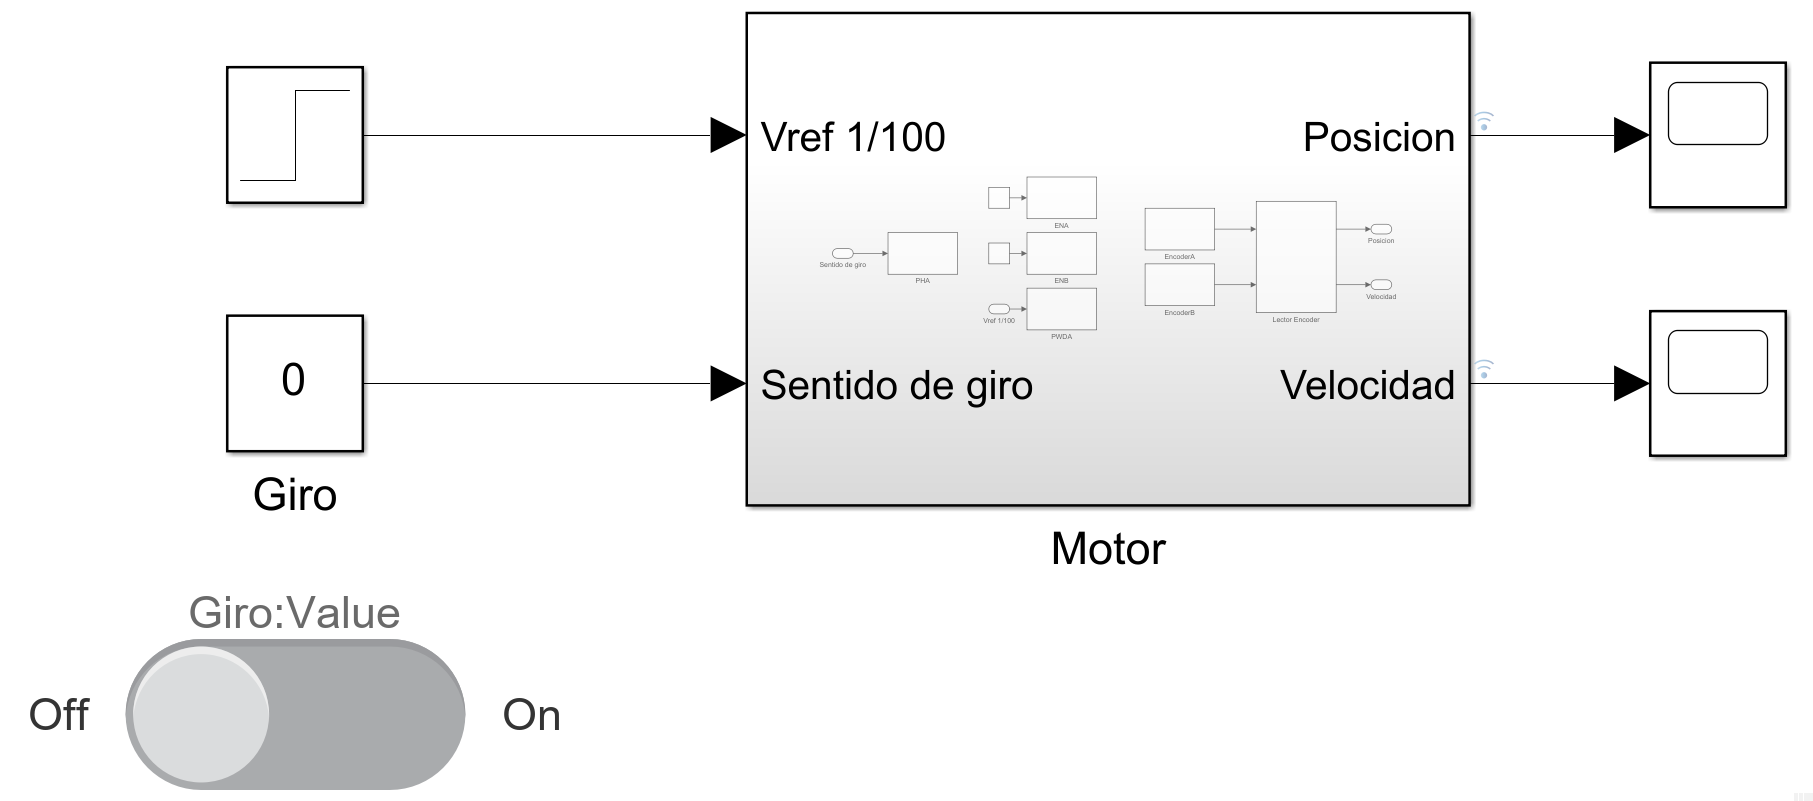
\includegraphics[height=4cm]{figs/motorbb.png}
	\caption{Modelo completo del motor en Simulink}
\end{figure}
\begin{figure}[h!]
	\centering
	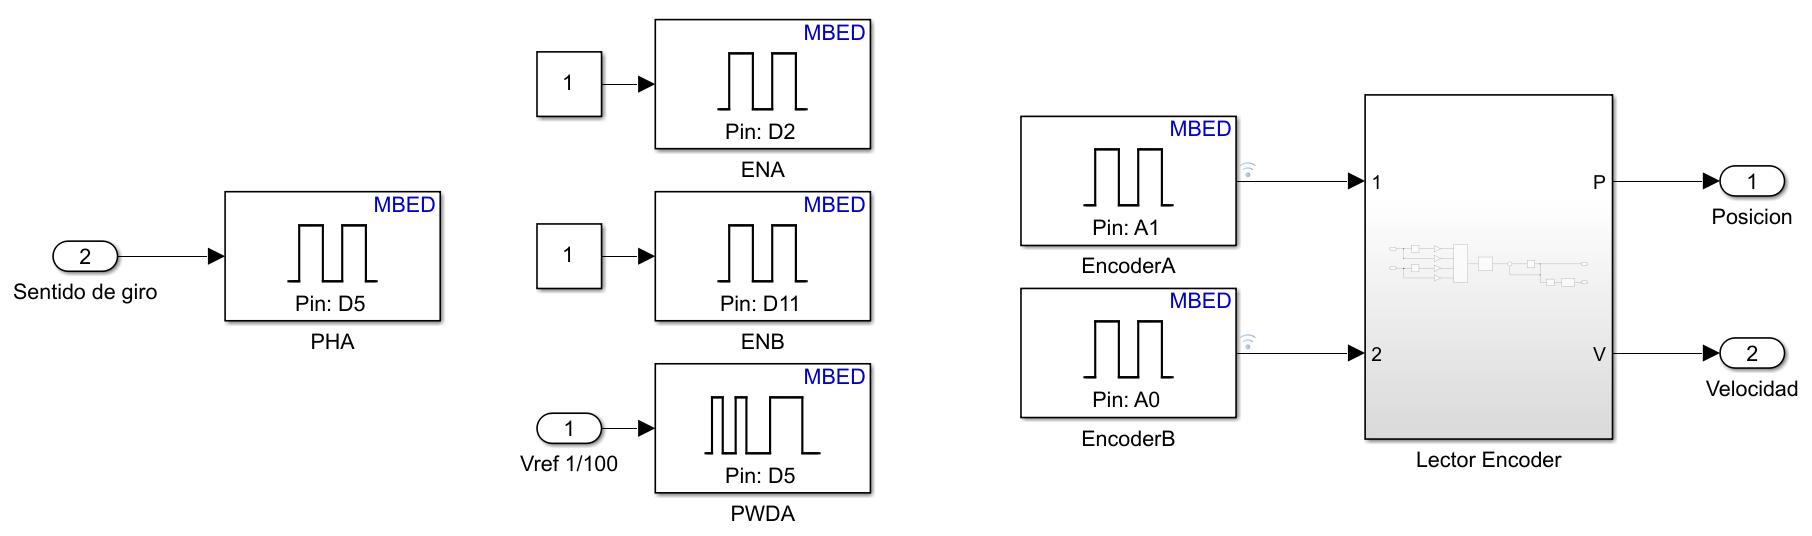
\includegraphics[height = 4cm]{figs/motorbb_inside.png}
	\caption{Bloque del motor}
\end{figure}
\begin{figure}[h!]
	\centering
	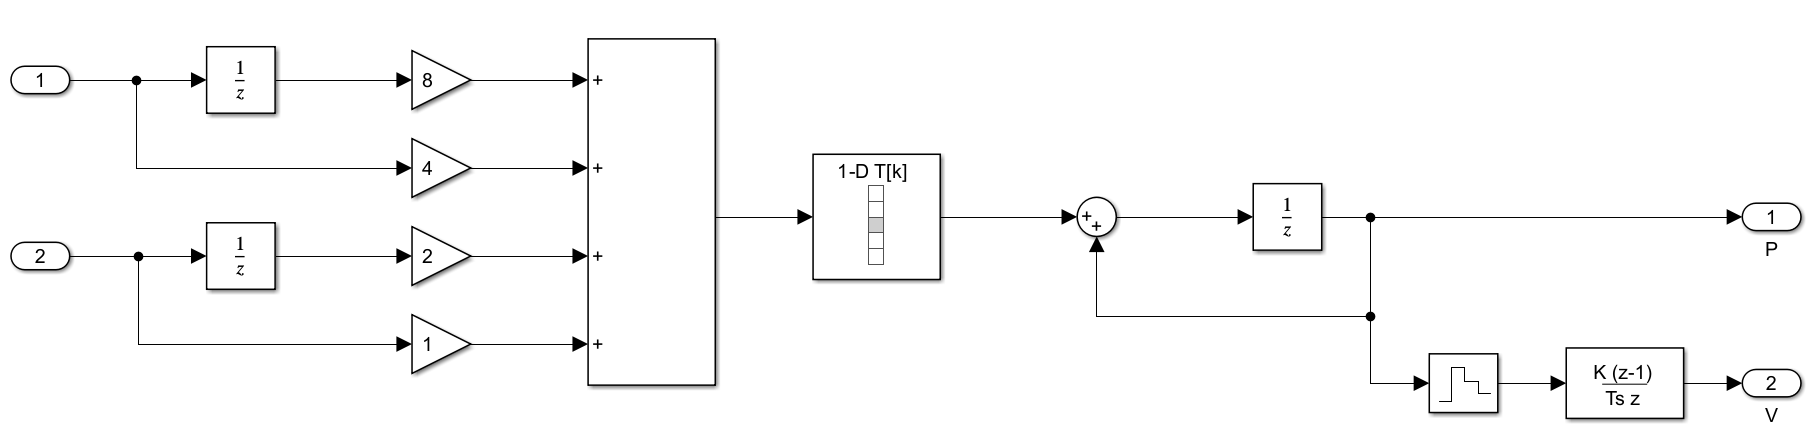
\includegraphics[height = 3.5cm]{figs/lector_encoders.png}
	\caption{Bloque de lectura de los encoders}
\end{figure}
\subsection{Identificación del motor}
\subsubsection{Cálculo de la funciones de respuesta}

A continuación se calcularán las funciones de respuesta de posición y velocidad del motor a partir del modelo en variables de estado y de la función de transferencia. 
Para el modelo en variables de estado, se tiene que 
\begin{align}
	\begin{bmatrix} \dot\theta \\ \dot\omega \end{bmatrix}  =  \begin{bmatrix} 0 & 1 \\ 0 & -p \end{bmatrix} \cdot \begin{bmatrix} \theta \\ \omega  \end{bmatrix} + \begin{bmatrix} 0 \\ k_e \end{bmatrix} V,
\end{align}
de donde se deducen las ecuaciones diferenciales 
\begin{align}
	\dot\theta(t) &= \omega(t) , \label{posdot} \\
	\dot\omega(t) &= -p \omega(t) + k_e V. \label{veldot}
\end{align}

Nótese que hemos definido la tensión de entrada $e(t)$ como una entrada escalón de valor $V$. Basta con resolver las ecuaciones anteriores imponiendo como condición inicial que $\omega(0) = 0, \theta(0) = 0$ para obtener las expresiones de respuesta:
\begin{align}
	\omega(t) &= V\frac{k_e}{p} - \frac{k_e }{p} e^{-p t},  \label{vel}\\
	\theta(t) &= V\frac{k_e}{p^2}e^{-p t} + V\frac{k_e}{p} t - V\frac{k_e}{p^2}.  \label{pos}
\end{align}

Inmediatamente se comprueba que la expresión \ref{pos} es la misma que la ecuación 3.14 del guion. 
Para calcularlo a partir de la función de transferencia de la posición

\begin{equation}
	\theta(s) = \frac{k_e}{s(s + p)} e(s)
\end{equation}
primero hay que calcular la transformada de Laplace de la entrada $e(t) = V$. Como V es una constante, fácilmente se obtiene $e(s) = \mathcal{L} (V) = \frac{V}{s}$. Una vez aplicada esta transformación, se pueden calcular las funciones de respuesta, resultando
\begin{align}
	\theta(t) = \mathcal{L}^{-1} [\theta(s)] &=  \frac{V  k_e }{p} t - \frac{V k_e}{p^2} + \frac{V k_e}{p^2} e^{-p t}, \\
	\omega(t) = \dot\theta(t) &= \frac{V  k_e}{p} - \frac{V k_e}{p} e^{-p t},
\end{align}
que son expresiones idénticas a las obtenidas a partir del modelo en variables de estado (ecuaciones \ref{pos} y \ref{vel}).

\subsubsection{Estimación de los valores de $k_e$ y $p$ del motor}
A continuación se va a tratar de obtener los parámetros del motor utilizando el modelo de Simulink de lazo abierto (Ver sección 1.1.2). 

\subsubsection{Comparación de los datos reales con el modelo de Simulink}
Se presenta en la siguiente figura el modelo desarrollado en Simulink, incluyendo los parámetros $p$ y $k_e$, construido a partir de las ecuaciones \ref{posdot} y \ref{veldot}. 
\begin{figure}[h!]
	\centering
	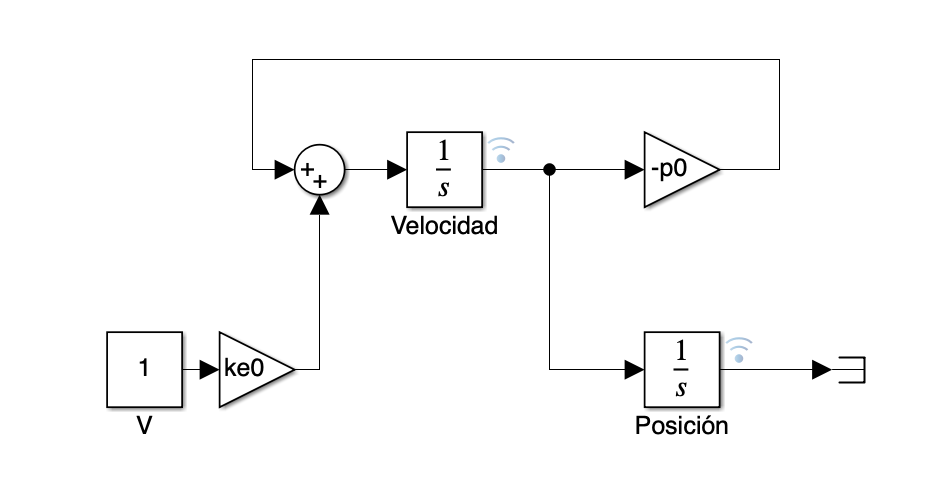
\includegraphics[height=5cm]{figs/pykesimulink}
	\caption{Modelo de Simulink para comprobar los valores obtenidos de $k_e$ y $p$}
\end{figure}

Del anterior modelo se observan las señales de salida de los integradores ``Velocidad" y ``Posición".  
Seguidamente se grafican estas señales junto a aquellas obtenidas inicialmente del motor para ciertos valores de tensión, por ejemplo 2, 6 y 12 V, 
a fin de observar discrepancias entre ellas. \\

Como se puede apreciar, tanto las señales del modelo como las medidas con el motor real coinciden, dando a entender que los parámetros estimados son adecuados para el motor. 



\section{Control del motor por realimentación de estados estimados}
\subsection{Modelo completo del motor}
En primer lugar, se procede a construir un modelo más completo que el modelo de motor ideal elaborado al final de la sección anterior, que incluya también un modelo para simular los encoders y la alimentación con señales de PWM. 
Para la lectura de los encoders, se reutilizará el bloque de lectura empleado para el manejo en lazo abierto. \\

\textbf{i) Modelo del sistema de alimentación}\\

El sistema de alimentación tratará de simular las señales de PWM (Pulse-Width Modulation) que recibe el motor desde la placa. Entonces, se empieza por construir un bloque que genere una señal con las mismas características.


\newpage



\section*{Anexo I: Código empleado para las prácticas}
\subsection*{Cálculo de funciones de transferencia}
\subsubsection*{ecs.m}
\begin{lstlisting}[language = MATLAB]
syms ke s p V w(t) theta(t) E(s) thetalap(t)
%Defino las ecuaciones diferenciales para resolver w (velocidad),
%theta (posición) y las resuelvo 
%Primero la velocidad
eqvel = diff(w, t) ==  -p*w + ke * V
wsol = dsolve(eqvel, w(0) == 0)

%Y luego la posición
eqpos = diff(theta, t) == wsol 
thetasol = dsolve(eqpos, theta(0) == 0) 

%Calculo la transformada de laplace de e(t) = V
E(s) = laplace(V, t, s) 
%Calculo la transformada inversa de la función de transferencia Th(s)
Th = ke /(s * (s + p)) * E(s) 
thetalap(t) = ilaplace(Th)

wlap = diff(thetalap(t), t)
\end{lstlisting}
\end{document}

